\documentclass[../../main.tex]{subfiles}
\begin{document}

{\bf [解答]}

与えられた曲線を
\begin{align}
  C: y = f(x) = \dfrac{1}{2}x + \sqrt{\left(\dfrac{1}{2}x\right)^2 + 2} \label{eq:1}
\end{align}
とする．

% TODO: y = f(x)の概形, P_1, P_2
\begin{figure}[htb]
  \centering
  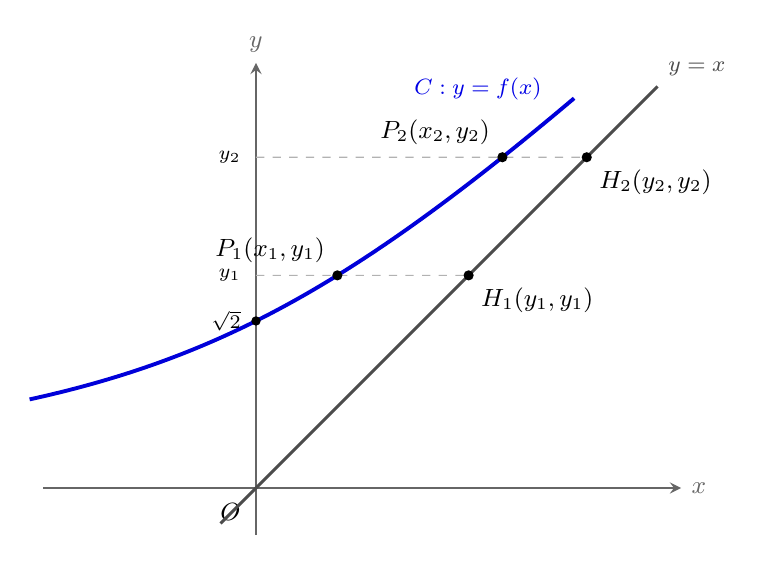
\begin{tikzpicture}[scale=1.5, >=stealth, every node/.style={font=\small}]

    % ============================================================
    % 1. 定数と座標計算
    % y - 2/y = x より
    % y1 = 1.8 => x1 = 1.8 - 2/1.8 ≈ 0.689
    % y2 = 2.8 => x2 = 2.8 - 2/2.8 ≈ 2.086
    % ============================================================
    \def\yA{1.8}
    \def\yB{2.8}
    \pgfmathsetmacro{\xA}{\yA - 2.0/\yA} % 0.6889
    \pgfmathsetmacro{\xB}{\yB - 2.0/\yB} % 2.0857

    \coordinate (O)  at (0, 0);
    \coordinate (P1) at (\xA, \yA);
    \coordinate (P2) at (\xB, \yB);
    \coordinate (H1) at (\yA, \yA);
    \coordinate (H2) at (\yB, \yB);

    % ============================================================
    % 3. 座標軸
    % ============================================================
    \draw[->, thick, gray!80!black] (-1.8, 0) -- (3.6, 0) node[right] {$x$};
    \draw[->, thick, gray!80!black] (0, -0.4) -- (0, 3.6) node[above] {$y$};
    \node[below left=2pt] at (O) {$O$};

    % ============================================================
    % 4. 直線 y = x と 漸近線
    % ============================================================
    % 直線 y = x
    \draw[line width=1.1pt, gray!60!black] (-0.3, -0.3) -- (3.4, 3.4)
    node[above right, font=\footnotesize] {$y = x$};

    % 漸近線 y = 0 (x < 0 側) と y = x (x > 0 側)
    % y = f(x)
    % x = y - 2/y を媒介変数表示で描画 (y: 0.7 -> 3.3)
    \draw[line width=1.4pt, blue!85!black, domain=0.75:3.3, samples=80, smooth, variable=\y]
    plot ({\y - 2.0/\y}, {\y});
    \node[blue!90!black, font=\footnotesize\bfseries, above left] at (2.5, 3.2) {$C: y = f(x)$};

    % y 切片 (0, sqrt(2))
    \node[circle, fill, inner sep=1.2pt] at (0, 1.4142) {};
    \node[left=2pt, font=\scriptsize] at (0, 1.4142) {$\sqrt{2}$};

    % ============================================================
    % 5. 補助線（水平線 y = y_1, y = y_2）
    % ============================================================
    \draw[dashed, gray!60] (0, \yA) -- (H1);
    \draw[dashed, gray!60] (0, \yB) -- (H2);
    \node[left=2pt, font=\scriptsize] at (0, \yA) {$y_1$};
    \node[left=2pt, font=\scriptsize] at (0, \yB) {$y_2$};

    % ============================================================
    % 6. 各点のプロットとラベル
    % ============================================================
    \node[circle, fill, inner sep=1.3pt] at (P1) {}; \node[above left=1pt] at (P1) {$P_1(x_1, y_1)$};
    \node[circle, fill, inner sep=1.3pt] at (P2) {}; \node[above left=1pt] at (P2) {$P_2(x_2, y_2)$};
    \node[circle, fill, inner sep=1.3pt] at (H1) {}; \node[below right=1pt] at (H1) {$H_1(y_1, y_1)$};
    \node[circle, fill, inner sep=1.3pt] at (H2) {}; \node[below right=1pt] at (H2) {$H_2(y_2, y_2)$};

  \end{tikzpicture}
  \caption{曲線 $y = f(x)$ の概形}
\end{figure}

\paragraph{(1)}

\begin{figure}[htb]
  \centering
  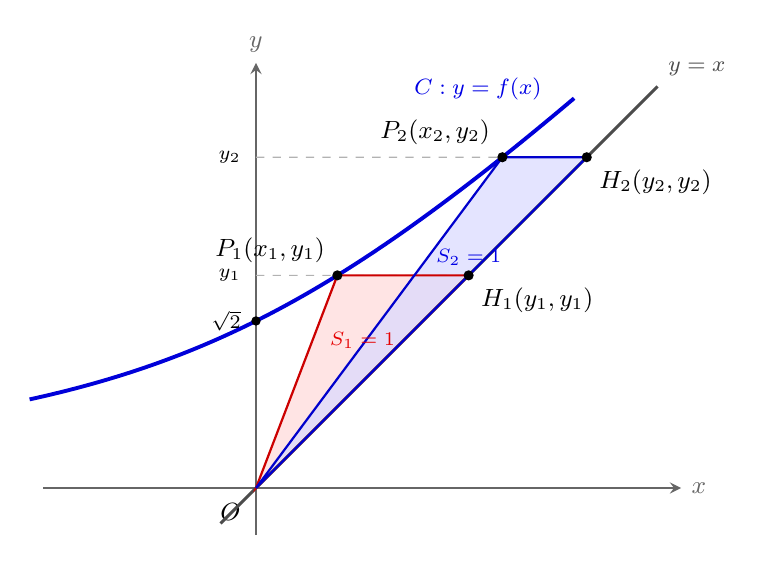
\begin{tikzpicture}[scale=1.5, >=stealth, every node/.style={font=\small}]

    % ============================================================
    % 1. 定数と座標計算
    % y - 2/y = x より
    % y1 = 1.8 => x1 = 1.8 - 2/1.8 ≈ 0.689
    % y2 = 2.8 => x2 = 2.8 - 2/2.8 ≈ 2.086
    % ============================================================
    \def\yA{1.8}
    \def\yB{2.8}
    \pgfmathsetmacro{\xA}{\yA - 2.0/\yA} % 0.6889
    \pgfmathsetmacro{\xB}{\yB - 2.0/\yB} % 2.0857

    \coordinate (O)  at (0, 0);
    \coordinate (P1) at (\xA, \yA);
    \coordinate (P2) at (\xB, \yB);
    \coordinate (H1) at (\yA, \yA);
    \coordinate (H2) at (\yB, \yB);

    % ============================================================
    % 2. 面積 S_1, S_2 の塗りつぶし
    % ============================================================
    \fill[red!15, opacity=0.7] (O) -- (P1) -- (H1) -- cycle;
    \fill[blue!15, opacity=0.7] (O) -- (P2) -- (H2) -- cycle;

    % ============================================================
    % 3. 座標軸
    % ============================================================
    \draw[->, thick, gray!80!black] (-1.8, 0) -- (3.6, 0) node[right] {$x$};
    \draw[->, thick, gray!80!black] (0, -0.4) -- (0, 3.6) node[above] {$y$};
    \node[below left=2pt] at (O) {$O$};

    % ============================================================
    % 4. 直線 y = x と 漸近線
    % ============================================================
    % 直線 y = x
    \draw[line width=1.1pt, gray!60!black] (-0.3, -0.3) -- (3.4, 3.4)
    node[above right, font=\footnotesize] {$y = x$};

    % 漸近線 y = 0 (x < 0 側) と y = x (x > 0 側)
    % y = f(x)
    % x = y - 2/y を媒介変数表示で描画 (y: 0.7 -> 3.3)
    \draw[line width=1.4pt, blue!85!black, domain=0.75:3.3, samples=80, smooth, variable=\y]
    plot ({\y - 2.0/\y}, {\y});
    \node[blue!90!black, font=\footnotesize\bfseries, above left] at (2.5, 3.2) {$C: y = f(x)$};

    % y 切片 (0, sqrt(2))
    \node[circle, fill, inner sep=1.2pt] at (0, 1.4142) {};
    \node[left=2pt, font=\scriptsize] at (0, 1.4142) {$\sqrt{2}$};

    % ============================================================
    % 5. 補助線（水平線 y = y_1, y = y_2）
    % ============================================================
    \draw[dashed, gray!60] (0, \yA) -- (H1);
    \draw[dashed, gray!60] (0, \yB) -- (H2);
    \node[left=2pt, font=\scriptsize] at (0, \yA) {$y_1$};
    \node[left=2pt, font=\scriptsize] at (0, \yB) {$y_2$};

    % OP1, OP2, P1H1, P2H2 の線分
    \draw[thick, red!80!black] (O) -- (P1) -- (H1) -- cycle;
    \draw[thick, blue!80!black] (O) -- (P2) -- (H2) -- cycle;

    % ============================================================
    % 6. 各点のプロットとラベル
    % ============================================================
    \node[circle, fill, inner sep=1.3pt] at (P1) {}; \node[above left=1pt] at (P1) {$P_1(x_1, y_1)$};
    \node[circle, fill, inner sep=1.3pt] at (P2) {}; \node[above left=1pt] at (P2) {$P_2(x_2, y_2)$};
    \node[circle, fill, inner sep=1.3pt] at (H1) {}; \node[below right=1pt] at (H1) {$H_1(y_1, y_1)$};
    \node[circle, fill, inner sep=1.3pt] at (H2) {}; \node[below right=1pt] at (H2) {$H_2(y_2, y_2)$};

    % 面積ラベル
    \node[red!90!black, font=\scriptsize\bfseries] at (0.9, 1.25) {$S_1 = 1$};
    \node[blue!90!black, font=\scriptsize\bfseries] at (1.8, 1.95) {$S_2 = 1$};

  \end{tikzpicture}
  \caption{曲線 $y = f(x)$ の概形と三角形 $\triangle OP_1H_1, \triangle OP_2H_2$}
\end{figure}

題意の直線は各々 $y=y_1, y=y_2$ であるから，$H_1(y_1, y_1), H_2(y_2,y_2)$ となる．
$\triangle OP_i H_i$ の面積 $S_i$ とすると，$S_1$はサラスの公式から
\begin{align}
  S_1
  &= \dfrac{1}{2} | x_1 y_1 - y_1 y_1 | \\
  &= \dfrac{1}{2} | y_1 | \left| \sqrt{\left(\dfrac{1}{2}x_1\right)^2+2} - \dfrac{1}{2}x_1 \right| \\
  &= \dfrac{1}{2} | y_1 | \dfrac{2}{|y_1|} = 1
\end{align}
となり，$S_1$ は $i$ によらない一定値となる．よって$S_2$も同じ値になり$\triangle OP_1 H_1 = \triangle OP_2 H_2$である．よって題意は示された．

\paragraph{(2)}

% TODO: y=f(x)
\begin{figure}[htb]
  \centering
  \begin{tikzpicture}[scale=1.75, >=stealth, every node/.style={font=\small}]

    % ============================================================
    % 1. 定数と座標計算
    % ============================================================
    \def\yA{1.8}
    \def\yB{2.8}
    \pgfmathsetmacro{\xA}{\yA - 2.0/\yA} % 0.6889
    \pgfmathsetmacro{\xB}{\yB - 2.0/\yB} % 2.0857

    \coordinate (O)  at (0, 0);
    \coordinate (P1) at (\xA, \yA);
    \coordinate (P2) at (\xB, \yB);
    \coordinate (H1) at (\yA, \yA);
    \coordinate (H2) at (\yB, \yB);

    % y 軸上の垂足 I_1, I_2
    \coordinate (I1) at (0, \yA);
    \coordinate (I2) at (0, \yB);

    % P1H1 と OP2 の交点 K
    \pgfmathsetmacro{\xK}{\yA * \xB / \yB} % ≈ 1.3408
    \coordinate (K) at (\xK, \yA);

    % ============================================================
    % 2. 2つの領域の斜線塗りつぶし
    % ============================================================
    % (A) 元の求める領域 S (OP1, OP2, 弧 P1P2) -> 青系の右上斜線
    \fill[pattern=north east lines, pattern color=blue!70, opacity=0.8]
    (O) -- (P1)
    -- plot[domain=\yA:\yB, samples=50, smooth, variable=\y] ({\y - 2.0/\y}, {\y})
    -- cycle;

    % (B) 等積変形後の領域 P2H2H1P1 (P1H1, H1H2, H2P2, 弧 P2P1) -> 橙/赤系の左上斜線
    \fill[pattern=north west lines, pattern color=red!75!black, opacity=0.7]
    (P1) -- (H1) -- (H2) -- (P2)
    -- plot[domain=\yB:\yA, samples=50, smooth, variable=\y] ({\y - 2.0/\y}, {\y})
    -- cycle;

    % ============================================================
    % 3. 座標軸
    % ============================================================
    \draw[->, thick, gray!80!black] (-0.8, 0) -- (3.6, 0) node[right] {$x$};
    \draw[->, thick, gray!80!black] (0, -0.4) -- (0, 3.6) node[above] {$y$};
    \node[below left=2pt] at (O) {$O$};

    % ============================================================
    % 4. 曲線 C と直線 y = x
    % ============================================================
    % 直線 y = x (H1, H2 を通る直線)
    \draw[line width=1.1pt, gray!45!black] (-0.2, -0.2) -- (3.3, 3.3)
    node[above right, font=\footnotesize] {$y = x$};

    % 曲線 C: x = y - 2/y
    \draw[line width=1.5pt, blue!85!black, domain=0.8:3.2, samples=70, smooth, variable=\y]
    plot ({\y - 2.0/\y}, {\y});
    \node[blue!90!black, font=\footnotesize\bfseries, above left] at (2.4, 3.1) {$C: x = y - \frac{2}{y}$};

    % ============================================================
    % 5. 境界線・補助線
    % ============================================================
    % 水平線 I1 - P1 - K - H1
    \draw[thick, gray!70!black] (I1) -- (H1);
    % 水平線 I2 - P2 - H2
    \draw[thick, gray!70!black] (I2) -- (H2);

    % 動径 OP1, OP2
    \draw[line width=1.2pt, blue!85!black] (O) -- (P1);
    \draw[line width=1.2pt, blue!85!black] (O) -- (P2);

    % H1H2 (直線 y = x の一部を強調)
    \draw[line width=1.3pt, red!85!black] (H1) -- (H2);
    \draw[line width=1.3pt, red!85!black] (P1) -- (H1);
    \draw[line width=1.3pt, red!85!black] (P2) -- (H2);

    % 等積変形を示す補助線 OH1, OH2
    \draw[dashed, gray!55] (O) -- (H1);
    \draw[dashed, gray!55] (O) -- (H2);

    % ============================================================
    % 6. 各点のプロットとラベル
    % ============================================================
    \node[circle, fill, inner sep=1.3pt] at (P1) {}; \node[above left=1pt] at (P1) {$P_1$};
    \node[circle, fill, inner sep=1.3pt] at (P2) {}; \node[above left=1pt] at (P2) {$P_2$};
    \node[circle, fill=red!85!black, inner sep=1.4pt] at (H1) {}; \node[below right=1pt, font=\footnotesize\bfseries, red!90!black] at (H1) {$H_1$};
    \node[circle, fill=red!85!black, inner sep=1.4pt] at (H2) {}; \node[below right=1pt, font=\footnotesize\bfseries, red!90!black] at (H2) {$H_2$};

    \node[circle, fill, inner sep=1.3pt] at (K) {}; \node[above right=1pt, font=\footnotesize] at (K) {$K$};

    \node[circle, fill, inner sep=1.2pt] at (I1) {}; \node[left=2pt] at (I1) {$I_1(y_1)$};
    \node[circle, fill, inner sep=1.2pt] at (I2) {}; \node[left=2pt] at (I2) {$I_2(y_2)$};

  \end{tikzpicture}
  \caption{求める領域 $S$（青斜線）と等積な図形 $P_2H_2H_1P_1$（赤斜線）の幾何学的対応}
  \label{fig:area_transformation_with_h1h2_shaded}
\end{figure}

$x_1<x_2$の時，図形の概要は上図のようになる．$H_1,H_2$から$y$軸におろした垂足を$I_1,I_2$とする．
$P_1H_1$ と $OP_2$ の交点を$K$とすると，求める面積$S$は
\begin{align}
  S = \triangle OP_1K + \text{図形}P_1KP_2 \label{eq:2}
\end{align}
である．(1)から$\triangle OP_1 H_1 =\triangle OP_2 H_2$だから
\begin{align}
  S
  &= \text{図形}P_1KP_2 + \triangle OP_1K + (\triangle OH_1K - \triangle OH_1K) \\
  &= \text{図形}P_1KP_2 + \triangle OP_1H_1 - \triangle OH_1K \\
  &= \text{図形}P_1KP_2 + \triangle OP_2H_2 - \triangle OH_1K \\
  &= \text{図形}P_1KP_2 + \text{図形} P_2KH_1P_1 \\
  &= \text{図形} P_2H_2H_1P_1
\end{align}
である．$x_1,x_2$の正負に応じて以下の$3$パターンが考えられる．

% TODO: x_2<0, x_1<0<x_2, 0<x_1の3つを横に並べる
\begin{figure}[htb]
  \centering
  \begin{tikzpicture}[scale=1.05, >=stealth, every node/.style={font=\scriptsize}]

    % =========================================================================
    % パターン 1: x_2 < 0 (2点とも y 軸の左側, y 切片 sqrt(2) ≈ 1.414 より下)
    % y1 = 0.8 => x1 = 0.8 - 2/0.8 = -1.7
    % y2 = 1.2 => x2 = 1.2 - 2/1.2 = -0.467
    % =========================================================================
    \begin{scope}[shift={(0, 0)}]
      \def\yA{0.8}
      \def\yB{1.2}
      \pgfmathsetmacro{\xA}{\yA - 2.0/\yA} % -1.7
      \pgfmathsetmacro{\xB}{\yB - 2.0/\yB} % -0.467

      \coordinate (O)  at (0, 0);
      \coordinate (P1) at (\xA, \yA);
      \coordinate (P2) at (\xB, \yB);
      \coordinate (H1) at (\yA, \yA);
      \coordinate (H2) at (\yB, \yB);
      \coordinate (I1) at (0, \yA);
      \coordinate (I2) at (0, \yB);

      % 面積 P2H2H1P1 (赤系ハッチング)
      \fill[pattern=north west lines, pattern color=red!75!black, opacity=0.7]
      (P1) -- (H1) -- (H2) -- (P2)
      -- plot[domain=\yB:\yA, samples=30, smooth, variable=\y] ({\y - 2.0/\y}, {\y})
      -- cycle;

      % 座標軸
      \draw[->, thick, gray!80!black] (-2.2, 0) -- (1.8, 0) node[right] {$x$};
      \draw[->, thick, gray!80!black] (0, -0.3) -- (0, 2.2) node[above] {$y$};
      \node[below left=1pt] at (O) {$O$};

      % y = x
      \draw[line width=0.8pt, gray!45!black] (-0.2, -0.2) -- (1.8, 1.8) node[above right] {$y=x$};

      % 曲線 C
      \draw[line width=1.2pt, blue!85!black, domain=0.65:1.6, samples=40, smooth, variable=\y]
      plot ({\y - 2.0/\y}, {\y});

      % 補助線
      \draw[thick, gray!60!black] (P1) -- (H1);
      \draw[thick, gray!60!black] (P2) -- (H2);
      \draw[line width=1.1pt, red!85!black] (H1) -- (H2);

      % 点プロット
      \node[circle, fill, inner sep=1.2pt] at (P1) {}; \node[above left=1pt] at (P1) {$P_1$};
      \node[circle, fill, inner sep=1.2pt] at (P2) {}; \node[above left=1pt] at (P2) {$P_2$};
      \node[circle, fill=red!85!black, inner sep=1.2pt] at (H1) {}; \node[red!85!black, below right=1pt] at (H1) {$H_1$};
      \node[circle, fill=red!85!black, inner sep=1.2pt] at (H2) {}; \node[red!85!black, below right=1pt] at (H2) {$H_2$};
      \node[circle, fill, inner sep=1.0pt] at (I1) {}; \node[right=1pt] at (I1) {$I_1$};
      \node[circle, fill, inner sep=1.0pt] at (I2) {}; \node[right=1pt] at (I2) {$I_2$};

      \node[below=8pt, font=\small\bfseries] at (-0.2, -0.3) {(a) $x_2 < 0$};
    \end{scope}

    % =========================================================================
    % パターン 2: x_1 < 0 < x_2 (P_1 が第2象限, P_2 が第1象限, y軸をまたぐ)
    % y1 = 1.0 => x1 = 1.0 - 2/1.0 = -1.0
    % y2 = 2.0 => x2 = 2.0 - 2/2.0 = 1.0
    % =========================================================================
    \begin{scope}[shift={(4.5, 0)}]
      \def\yA{1.0}
      \def\yB{2.0}
      \pgfmathsetmacro{\xA}{\yA - 2.0/\yA} % -1.0
      \pgfmathsetmacro{\xB}{\yB - 2.0/\yB} % 1.0

      \coordinate (O)  at (0, 0);
      \coordinate (P1) at (\xA, \yA);
      \coordinate (P2) at (\xB, \yB);
      \coordinate (H1) at (\yA, \yA);
      \coordinate (H2) at (\yB, \yB);
      \coordinate (I1) at (0, \yA);
      \coordinate (I2) at (0, \yB);
      \coordinate (L)  at (0, 1.4142);

      % 面積 P2H2H1P1 (赤系ハッチング)
      \fill[pattern=north west lines, pattern color=red!75!black, opacity=0.7]
      (P1) -- (H1) -- (H2) -- (P2)
      -- plot[domain=\yB:\yA, samples=40, smooth, variable=\y] ({\y - 2.0/\y}, {\y})
      -- cycle;

      % 座標軸
      \draw[->, thick, gray!80!black] (-1.6, 0) -- (2.4, 0) node[right] {$x$};
      \draw[->, thick, gray!80!black] (0, -0.3) -- (0, 2.5) node[above] {$y$};
      \node[below left=1pt] at (O) {$O$};

      % y = x
      \draw[line width=0.8pt, gray!45!black] (-0.2, -0.2) -- (2.3, 2.3) node[above right] {$y=x$};

      % 曲線 C
      \draw[line width=1.2pt, blue!85!black, domain=0.8:2.3, samples=50, smooth, variable=\y]
      plot ({\y - 2.0/\y}, {\y});

      % 補助線
      \draw[thick, gray!60!black] (P1) -- (H1);
      \draw[thick, gray!60!black] (I2) -- (H2);
      \draw[line width=1.1pt, red!85!black] (H1) -- (H2);

      % 点プロット
      \node[circle, fill, inner sep=1.2pt] at (P1) {}; \node[above left=1pt] at (P1) {$P_1$};
      \node[circle, fill, inner sep=1.2pt] at (P2) {}; \node[above left=1pt] at (P2) {$P_2$};
      \node[circle, fill=red!85!black, inner sep=1.2pt] at (H1) {}; \node[red!85!black, below right=1pt] at (H1) {$H_1$};
      \node[circle, fill=red!85!black, inner sep=1.2pt] at (H2) {}; \node[red!85!black, below right=1pt] at (H2) {$H_2$};
      \node[circle, fill, inner sep=1.0pt] at (I1) {}; \node[below right=1pt] at (I1) {$I_1$};
      \node[circle, fill, inner sep=1.0pt] at (I2) {}; \node[left=1pt] at (I2) {$I_2$};
      \node[circle, fill, inner sep=1.0pt] at (L) {}; \node[left=1pt] at (L) {$L$};

      \node[below=8pt, font=\small\bfseries] at (0.3, -0.3) {(b) $x_1 < 0 < x_2$};
    \end{scope}

    % =========================================================================
    % パターン 3: 0 < x_1 (2点とも y 軸の右側)
    % y1 = 1.8 => x1 = 1.8 - 2/1.8 ≈ 0.689
    % y2 = 2.8 => x2 = 2.8 - 2/2.8 ≈ 2.086
    % =========================================================================
    \begin{scope}[shift={(9.2, 0)}]
      \def\yA{1.8}
      \def\yB{2.8}
      \pgfmathsetmacro{\xA}{\yA - 2.0/\yA} % 0.689
      \pgfmathsetmacro{\xB}{\yB - 2.0/\yB} % 2.086

      \coordinate (O)  at (0, 0);
      \coordinate (P1) at (\xA, \yA);
      \coordinate (P2) at (\xB, \yB);
      \coordinate (H1) at (\yA, \yA);
      \coordinate (H2) at (\yB, \yB);
      \coordinate (I1) at (0, \yA);
      \coordinate (I2) at (0, \yB);

      % 面積 P2H2H1P1 (赤系ハッチング)
      \fill[pattern=north west lines, pattern color=red!75!black, opacity=0.7]
      (P1) -- (H1) -- (H2) -- (P2)
      -- plot[domain=\yB:\yA, samples=30, smooth, variable=\y] ({\y - 2.0/\y}, {\y})
      -- cycle;

      % 座標軸
      \draw[->, thick, gray!80!black] (-0.6, 0) -- (3.2, 0) node[right] {$x$};
      \draw[->, thick, gray!80!black] (0, -0.3) -- (0, 3.2) node[above] {$y$};
      \node[below left=1pt] at (O) {$O$};

      % y = x
      \draw[line width=0.8pt, gray!45!black] (-0.2, -0.2) -- (3.0, 3.0) node[above right] {$y=x$};

      % 曲線 C
      \draw[line width=1.2pt, blue!85!black, domain=1.2:3.1, samples=40, smooth, variable=\y]
      plot ({\y - 2.0/\y}, {\y});

      % 補助線
      \draw[thick, gray!60!black] (I1) -- (H1);
      \draw[thick, gray!60!black] (I2) -- (H2);
      \draw[line width=1.1pt, red!85!black] (H1) -- (H2);

      % 点プロット
      \node[circle, fill, inner sep=1.2pt] at (P1) {}; \node[above left=1pt] at (P1) {$P_1$};
      \node[circle, fill, inner sep=1.2pt] at (P2) {}; \node[above left=1pt] at (P2) {$P_2$};
      \node[circle, fill=red!85!black, inner sep=1.2pt] at (H1) {}; \node[red!85!black, below right=1pt] at (H1) {$H_1$};
      \node[circle, fill=red!85!black, inner sep=1.2pt] at (H2) {}; \node[red!85!black, below right=1pt] at (H2) {$H_2$};
      \node[circle, fill, inner sep=1.0pt] at (I1) {}; \node[left=1pt] at (I1) {$I_1$};
      \node[circle, fill, inner sep=1.0pt] at (I2) {}; \node[left=1pt] at (I2) {$I_2$};

      \node[below=8pt, font=\small\bfseries] at (1.2, -0.3) {(c) $0 < x_1$};
    \end{scope}

  \end{tikzpicture}
  \caption{$x_1, x_2$ の符号による図形 $P_2H_2H_1P_1$（斜線部）の3つの配置パターン}
  \label{fig:three_cases_cross_section_area}
\end{figure}

それぞれ式に起こすと
\begin{align}
  S=
  \begin{cases}
    \text{台形} I_2I_1H_1H_2 + \text{図形}I_2I_1P_1P_2 & (x_2 < 0) \\
    \text{台形} I_2I_1H_1H_2 + \text{図形}P_1I_1L - \text{図形}P_2I_2L & (x_1<0<x_2) \\
    \text{台形} I_2I_1H_1H_2 - \text{図形}I_2I_1P_1P_2 & (0<x_1)
  \end{cases}
\end{align}
だが，これは符号付きの面積を考えると
\begin{align}
  S = \text{台形} I_2I_1H_1H_2 - \int_{y_1}^{y_2} x dy \label{eq:3}
\end{align}
と統一的に扱える．以下個別に項を計算する．

$\text{図形}I_2I_1P_1P_2$の面積を求めるため，$y=f(x)$を逆にとくと
\begin{align}
  y - \dfrac{1}{2}x = \sqrt{\left(\dfrac{1}{2}x\right)^2 + 2}
\end{align}
であり，図から $y - \dfrac{1}{2}x > 0$ だから両辺 $0$ 以上なので2乗して
\begin{align}
  y^2 - xy = 2 \implies x = \dfrac{y^2 - 2}{y} = y - \dfrac{2}{y} \label{eq:4}
\end{align}
である．

従って
\begin{align}
  \text{図形}I_2I_1P_1P_2
  & = \int_{y_1}^{y_2} x dy \\
  & = \int_{y_1}^{y_2} \left(y-\dfrac{2}{y}\right) dy \\
  & = \left[ \dfrac{1}{2}y^2 - 2\log y \right]_{y_1}^{y_2} \\
  & = \dfrac{1}{2}\left(y_2^2-y_1^2\right) - 2\log\dfrac{y_2}{y_1} \label{eq:5}
\end{align}
である．また，
\begin{align}
  \text{台形} I_2I_1H_1H_2
  & = \dfrac{1}{2}(|H_1I_1|+|H_2I_2|)(I_2-I_1)
  = \dfrac{1}{2}(y_1 + y_2)(y_2 - y_1)
  = \dfrac{1}{2}(y_2^2 - y_1^2) \label{eq:6}
\end{align}
である．

\cref{eq:5,eq:6}を\cref{eq:3}に代入して求める面積は
\begin{align}
  S
  &= \text{(台形)} - \text{(積分)} \\
  &= \dfrac{1}{2}(y_2^2 - y_1^2) - \left[ \dfrac{1}{2}y^2 - 2\log y \right]_{y_1}^{y_2} \\
  &= 2\log\dfrac{y_2}{y_1}
\end{align}
である．

% TODO: 別解として，x = cosh tと置換すれば普通にxについて積分できる

\end{document}
